\documentclass{jsarticle}

% パッケージ
\usepackage[dvipdfmx]{graphicx}
\usepackage{url}
\begin{document}

% 脚注フォーマット
\renewcommand\thefootnote{\arabic{footnote})}


% 表紙

{\Large \today 提出}\\ % 提出日

\begin{center}
\vspace{120truept}
{\huge 平成28年度 卒業論文\\[10mm]
IPOほにゃらら}\\ % タイトル
\vspace{10truept}
{\Large サブタイトル}\\ % サブタイトル(なければコメントアウト)
\vspace{120truept}
{\huge 学籍番号 07-150041}\\ % 学籍番号
\vspace{50truept}
{\huge 東京大学経済学部経済学科\\[50truept]
岡部 匡志}\\ % 著者

\end{center}
\newpage
\begin{center}
{\Large IPOほにゃらら}\\ % タイトル
\end{center}

% 目次
\tableofcontents
\vspace{120truept}
% 本文
\section{はじめに(要更新)}
本稿では、日本の新規株式公開\footnote[1]{Initial Public Offering。以下、 「IPO」とする。}市場において、直近の数社のパフォーマンスがアンダープライシング\footnote[2]{\{(初値) - (公開価格)\} / (公開価格)\} として示される。100\%からの乖離を、初期収益率・初期乖離率と呼ぶこともある。ここで、公開価格とは、「IPO直前に希望する投資家に対して新規公開予定の株式を売却する際の価格(岡村 2011\cite{okamura})である。また、本稿では初値として、マーケットで付けられた、取引初日における最初の価格を用いる。}にどのような影響を及ぼしているのかについて考察を行う。
\section{IPOにおけるアンダープライシング}
\subsection{アノマリーとしてのアンダープライシング}
アンダープライシング自体は、国内外で一種の経済学的アノマリー\footnote[3]{例えば、辰巳・桂山 2005\cite{tatsumi}に、ファイナンス分野で知られるアノマリーが詳しい。}として知られており、表\ref{around_world}の通り、国内外でその存在が継続的に確認されている。 \par
公開価格には企業のファンダメンタルズが適切に評価されており、初値は株式市場において効率的に形成されると想定するなら、このような現象が継続的に発生しているという事実は、アノマリーと言わざるを得ない。この状況の下では、投資家は、公開価格で株式を購入し、数週間後の上場後に株式を売却するだけで、高い収益率を得られる。実際に、IPO時において、アンダーライター\footnote[4]{ここでは、株式の発行・売出しに際し、株式を売れ残った際に発行者や所有者から取得する者のことであり、日本国内においては、IPOを主導する主幹事証券会社を中心としたシンジゲート団のことを指す。}が実施する公募への抽選には個人投資家からの注文が殺到する。

\begin{table}[h]
	\caption{世界各国における初期収益率の算術平均。
	Loughran et el.(1994, updated 2015) \cite{Loughran}より一部抜粋。}
	\label{around_world}
	\centering
	\begin{tabular}{cccc}
		\hline
		国名&サンプル数&期間&平均初期収益率(100\%からの乖離) \\
		\hline \hline
		英国&4,932&1959-2012&16.0\% \\
		韓国&1,758&1980-2014& 58.8\% \\
		シンガポール&609&1973-2013&25.8\% \\
		タイ&500&1987-2012&35.1\%\\
		台湾 &1,620 &1980-2013&38.1\% \\
		中国&2,512&1990-2013&118.4\%\\
		ドイツ&736&1978-2011&24.2\% \\
		日本&3,236&1970-2013&41.7\% \\
		フランス & 697 & 1983-2010 & 10.5\% \\
		米国&12,702&1960-2012&16.9\%\\
		\hline
	\end{tabular}
\end{table}


\subsection{アンダープライシングをめぐる仮説}
アンダープライシングは、IPOにおけるアノマリー、あるいは、ある種のマーケットの歪みとして、研究者や投資家たちの強い関心を集めてきた。特に研究面の関心は、アンダープライシングを合理的に説明する決定メカニズムの解明に向けられており、現在に至るまで数多くの仮説が提案されてきたと言える。\par
既存研究における、アンダープライシングの決定メカニズムをめぐる仮説は、大きく2つに分類出来るだろう。すなわち、アノマリーの原因を情報の非対称性に求めるものと、各プレーヤーの限定合理性に求めるものである。\par
前者の仮説については、岡村 2011\cite{okamura}によく整理されている。本稿では名前を列挙するに留めるが、「逆選択回避仮説(別名:Winner's Curse)」「エージェンシー仮説」「情報検事仮説」など、それぞれ、アンダーライターが公開価格を意図的に引き下げる誘引を持つことを説明している。\par

また、アンダーライターではなく、投資家の側に、公開前需要の申告\footnote[5]{日本の株式市場で実施されているブックビルディング方式における、公開価格決定プロセスの一部。}に際して、株式の市場価格の観察不能性によるリスクの存在から、公開価格を押し下げる誘引が存在することを説明した研究として、池田 (2013)\cite{ikeda}がある。\par

一方で、近年の行動経済学・行動ファイナンスの発展に伴い、プレーヤーの限定合理性を導入してアンダープライシングを説明しようとする研究が展開されている。その代表的なものとして、「後の投資家は、それまでの他の投資家が行った購入意思決定を意思決定に反映させ、自らの都合に合わせて情報を無視、あるいは軽視し、先の投資家に追随する」という、いわゆる情報カスケード効果\footnote[6]{Welch (1992)\cite{Welch}がその端緒とされている。}が挙げられるだろう。\par




現実的な解釈としては、「どの仮説が正しい/誤っている」という問題ではなく、それぞれの仮説が折り重なって実際のアンダープライシングが形成されている、ということになる。以下、本稿では、図\ref{transition}のように、アンダープライシングの程度が時期によって大きく異なっていることに注目し、情報カスケード効果を想定した、マーケット・コンディションの存在と、その解明について論じていく。

\section{リサーチ・デザイン}
\subsection{本研究の目的と意義}
金子 (2009)\cite{kaneko}も指摘する通り、「間もなく発行される株式をいくら以下なら購入してもよいかを考える際に、投資家がおそらくもっとも参考にしたいと考える現在の株価が、PO(著者注:すでに株式を公開している企業が一般投資家向けに株式を発行すること)の方は存在するがIPOの方は存在しない」(p.84)ことが、IPOの初値形成における固有の事情と言える。\par
それでは、投資家は何を参考に、情報が不足する株式の購入意思決定を行っているのだろうか。\par
本稿では、直近の他のIPOにおけるパフォーマンスが、当該IPOのパフォーマンスに影響を与えると考える。すなわち、直近のIPOにおいて高いアンダープライシングが観測されたとき、投資家は自分が持つ、当該企業についてのファンダメンタルズの情報を軽視し、「今はマーケット・コンディションが良い」と考えることで、マーケットにおいて高い価格を付けるのではないか、という仮説である。\par
独自のマーケット・コンディション指数を定義し、アンダープライシングへの回帰を行った研究として、Derrien (2005)\cite{Derrien}が挙げられる。Derrienは、マーケット・コンディションを、IPO企業の属する業種インデックスの上場前3ヶ月間のパフォーマンスと定義している。本稿では、マーケット・コンディション指数を積極的に設定することはせず、IPO時における直近の数件のアンダープライシングの多寡それ自体が、マーケット・コンディションとして機能していると考える。\par
<要修正>著者の知る限りにおいて、アンダープライシングを時系列的に捉えた研究は存在せず、本稿がその端緒となれば幸いである。\par
仮説の検証には、AR(p)モデルを用い、AIC(赤池情報基準)を用いて適切なラグ次数を求めた後、ほにゃほにゃ統計量を用いて単位根の検定を行う。\par
また、インデックスを共変量に加えたモデルも用意し、IPOマーケットが通常の株式市場とどういった関係にあるか、も考察する。

\subsection{データ・ソース}
前章で提示した仮説を検証するために、1997年9月に上場した株式会社フォトロン(現:株式会社イマジカ・ロボット ホールディングス)から、2016年12月に上場した株式会社グッドコムアセットまでの、計1962社をサンプル・データとして用いる。\footnote[7]{データは、\url{https://github.com/M-okb/IPO_analysis}で公開している。用いたデータの内、1997年から2009年のものについては、Kaneko and Pettway’s Japanese IPO Database(\url{http://www.fbc.keio.ac.jp/~kaneko/KP-JIPO/top.htm})で公開されているデータから、2010年以降のものについては、総合投資情報サイト(\url{http://www.traders.co.jp/})、Yahoo finance(\url{http://stocks.finance.yahoo.co.jp/})から取得した。ここに感謝の意を表します。}\par
なお、上場中止・上場延期になったもの(例:株式会社ZMP)や、J-REIT(例:星野リゾート・リート投資法人)などは扱っていない。\par
\subsection{データの特徴}
\subsubsection{IPO件数とアンダープライシング}
前述したとおり、図\ref{transition}ように、年度によってアンダープライシングの度合いは大きく異なる。具体的には、2000年\footnote[8]{IPOバブル崩壊の年である。政府による起業支援や、ストック・オプションの規制緩和などを受け、情報通信業系の企業を中心に市況が活性化したが、2000年3月、光通信の不正をキッカケにネット関連銘柄の株価は大きく値下げした。}前後で大きく下落している他、2005年がピークとなっており、2010年周辺では100\%は割らないとは言え、低迷している。\par
全てのアンダープライシングをヒストグラムに取ったのが図\ref{hist}であり、値は正規分布せず、右に裾野の広い分布となっている。
図\ref{loghist}に、それを対数表示した。既存研究では、アンダープライシングを100分率で表示し、それを被説明変数に用いることが多かったが、本稿では100分率でなく、比率を自然対数で表示したものを用いる。\par
また、アンダープライシングの5年おきの基本統計量の推移を表\ref{stats}に示した。どの時代でも、おおよそ、25\%tileを境目として、初期収益率がプラスとなることが分かる。\par
年度別のIPO数は図\ref{fig:year}のようになっており、多い年では、少ない年の10倍近くのIPOがある。こちらは、アンダープライシングとは異なり、IPOバブル崩壊の影響は限定的であるが、2008年のリーマン・ショックの影響を大きく受けているように見受けられる。
\subsubsection{上場時の企業年齢}
会社設立から、上場までの所要年数を図にプロットした。大きく変化がないといいなぁ〜!


\subsubsection{業種}


\subsubsection{主幹事}
\subsubsection{市場}



\subsection{モデルの構造と想定される結果}
数式。
変数の説明。

\section{実証分析の結果}
\section{総括と今後の課題}

\newpage

\begin{figure}[p]
  \begin{center}
  \caption{アンダープライシングの年度別平均値の推移(1997〜2016) 後述のデータより著者作成}
    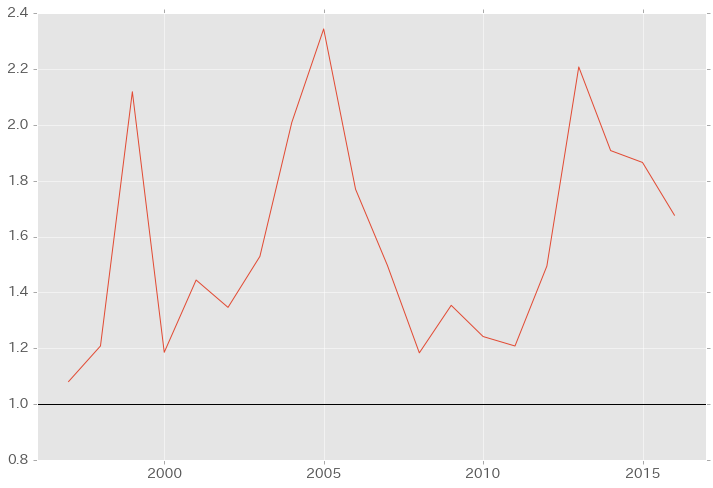
\includegraphics[clip,width=14cm]{./transition.png}
    \label{transition}
  \end{center}
\end{figure}


\begin{figure}[p]
  \begin{center}
  \caption{アンダープライシング(1997〜2016)の分布ヒストグラム}
    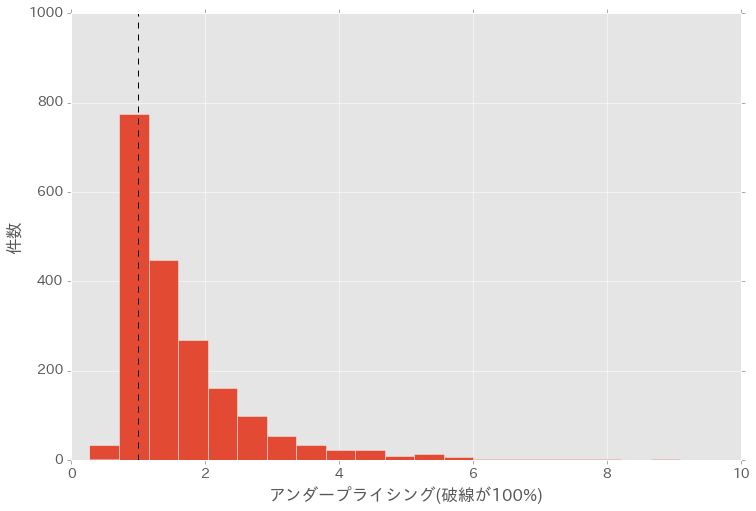
\includegraphics[clip,width=14cm]{./hist.png}
    \label{hist}
  \end{center}
\end{figure}

\begin{figure}[p]
  \begin{center}
  \caption{アンダープライシング(1997〜2016)の対数分布ヒストグラム}
    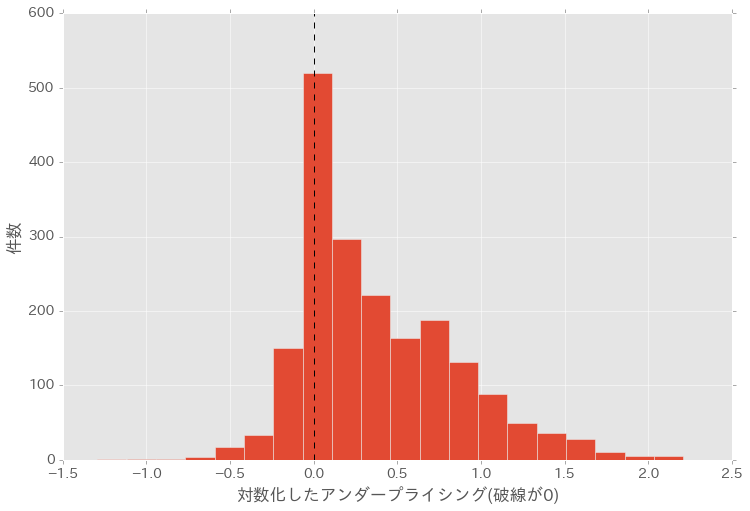
\includegraphics[clip,width=14cm]{./loghist.png}
    \label{loghist}
  \end{center}
\end{figure}

\begin{figure}[p]
  \begin{center}
  \caption{アンダープライシングの基本統計量の5年おきの推移(1997〜2016)}
\begin{tabular*}{120mm}{@{\extracolsep{\fill}}c|ccccc}

\hline
\  & 総計 &  1997 &  2002&   2007  & 2012 \\
\hline \hline
件数 &1962 & 606 & 766 & 249 & 341 \\
\hline
標準偏差&       0.990  &0.911  &1.080 & 0.601 & 1.005 \\
\hline
平均値   &  1.647 & 1.417 & 1.836 & 1.357 & 1.840 \\
\hline
最小値    &     0.275 & 0.275 & 0.583 & 0.571&  0.531 \\
25\%tile   &       1.026 & 1.000  &1.094 & 0.941 & 1.089 \\
50\%tile    &      1.271&  1.115 & 1.472 & 1.077  &1.486 \\
75\%tile     &     1.999 & 1.500 & 2.183  &1.694 & 2.294 \\
最大値  &   9.091 & 9.091&  8.727 & 4.086 & 5.625 \\
\hline
	\end{tabular*}
	\label{stats} 
  \end{center}
\end{figure}

\begin{figure}[p]
  \begin{center}
  \caption{IPO数の年度別推移(1997〜2016) 著者作成}
  \begin{tabular}{c}
  \begin{minipage}{0.5\hsize}
  \begin{center}
    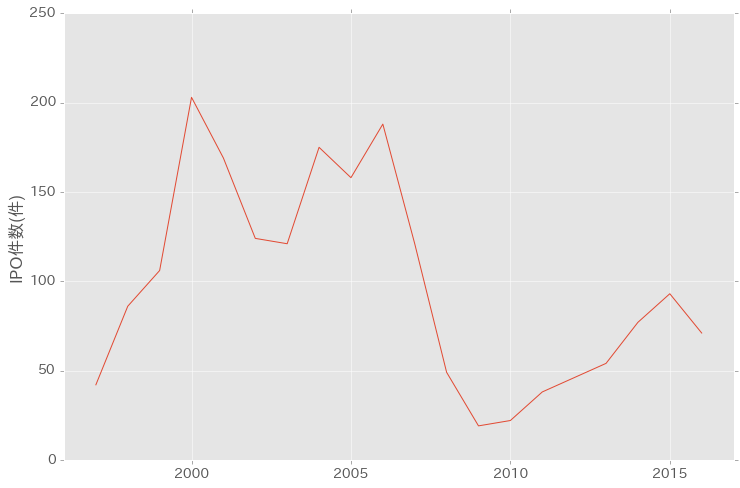
\includegraphics[clip,width=9cm]{./year_count.png}
     \end{center}
\end{minipage}
\begin{minipage}{0.5\hsize}
\begin{center}
    \label{fig:year}
\begin{tabular}{cc|cc}
		\hline
		年度 & 件数 & 年度 & 件数 \\
		\hline \hline
1997  &   42 & 2007  &  121\\
1998  &   86 & 2008   &  49\\
1999   & 106 & 2009  &   19\\
2000 &   203 & 2010  &   22\\
2001  &  169 & 2011   &  38\\
2002 &   124 & 2012  &   46\\
2003 &   121 & 2013 &    54\\
2004 &   175 & 2014   &  77\\
2005 &   158 & 2015  &   93\\
2006  &  188 & 2016 &    71\\
		\hline
	\end{tabular} 
	 \end{center}
	\end{minipage}
	  \end{tabular}
	    \end{center}
\end{figure}



\begin{thebibliography}{99}
\bibitem{okamura} 岡村秀夫 (2011)「IPO研究の展開」, 『商学論究, 58(3):45-65』
\bibitem{tatsumi} 辰巳憲一・桂山靖代 (2005)「IPOリターン・リバーバル —初取引日前後IPOパフォーマンスのアノマリー分析—」, 『学習院大学 経済論集, 第42巻 第3号』
\bibitem{Loughran} Loughram, T., Ritter, J. and Rydqvist, K. (1994) "Initial Public Offering: International Insights," Pacific-Basin Finance Journal 2, 165-199. (updated 2015)
\bibitem{ikeda} 池田直史 (2013) 「IPOの株価観察不能性と正の初期収益率」, 『金融経済研究, 第35号 34-51』
\bibitem{Welch} Welch, I. (1992) "Sequential Sales, Learning, and Cascades," The Journal of FINANCE 47, 695-732.
\bibitem{Derrien} Derrien, F. (2005) "IPO Pricing in "Hot" Market Conditions: Who Leaves Money On the Table?," Journal of Finance 60, 487-615
\bibitem{kaneko} 金子隆 (2009) 「IPOの過小値付け現象 −新しい解釈の試み−」, 『三田商学研究 第52巻 第2号』
\end{thebibliography}
\end{document}